\chapter{Reelle Rekonstruktion}
\label{sec:real} 

Der entwickelte Szenenrekonstrukionsalgorithmus wird im folgenden anhand eines realen Stereoaufbau getestet. Da das Arbeiten mit realen Bilddaten bestimmte Fehleranfälligkeiten aufweist, wird in diesem Kapitel Hauptsächlich drauf eingegangen, um welche Fehler es sich handelt, was ihre Auswirkungen sind und wie man ihnen entgegenwirken kann. Hierzu wurde der Ursprüngliche Algorithmus um bestimmte Funktionen erweitert, welche im Verlauf des Kapitels genau erläutert werden. Abbildung \ref{fig:ArbeitsProzessReell} zeigt den Ablauf für die Reelle Rekonstruktion. \\


\begin{minipage}{\linewidth}
	\centering
	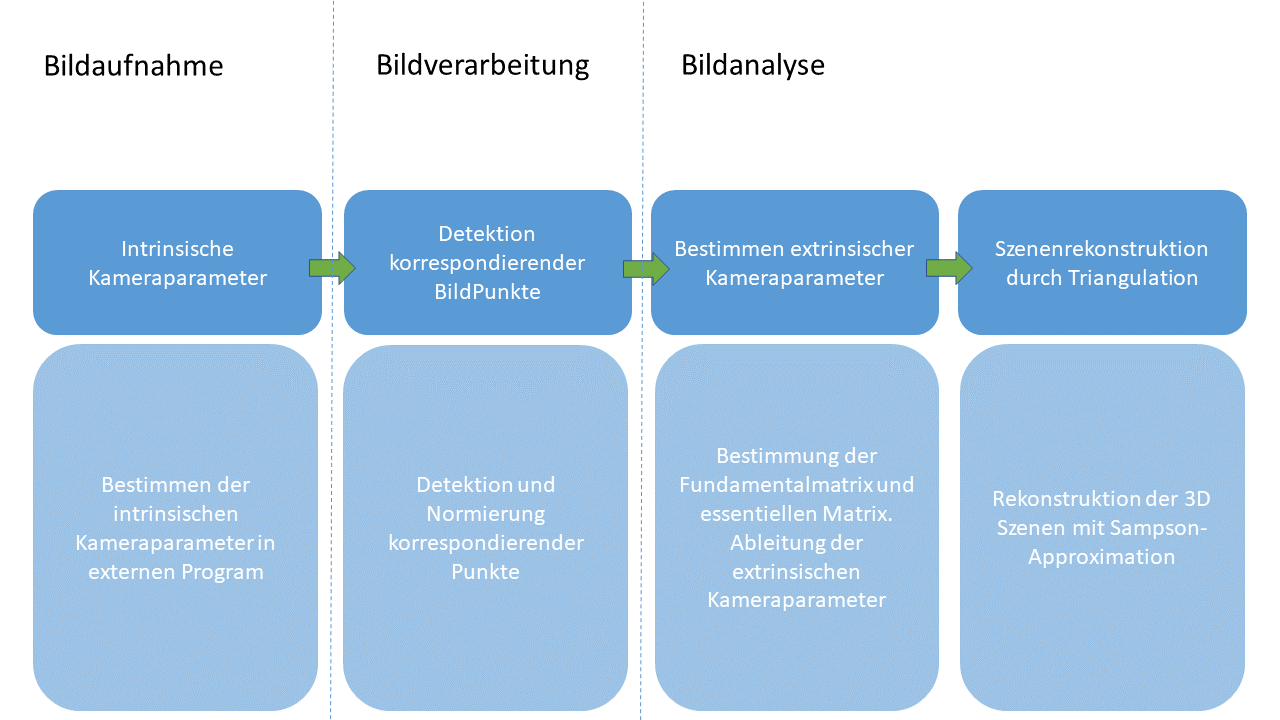
\includegraphics[width=1.\linewidth]{images/NEU_real_Arbeitsprozess.png}
	\captionof{figure}{Ablaufdiagramm für die reelle Rekonstruktion}
	\label{fig:ArbeitsProzessReell}
\end{minipage}\\ \\

Zu aller erst wird der Stereoaufbau vorgestellt. Danach folgt die Korrespondenzanalyse, in welcher zwei Möglichkeiten aufgeführt werden, wie die Korrespondierenden Punkte aus den Bildern gewonnen werden. Der normierte-acht-Punkt-Algorithmus, stellt eine für reale Bilddaten leicht veränderte Fassung des bereits bekannten acht-Punkte-Algorithmus vor. Danach werden die Singulärwerte der aus realen Daten bestimmten Fundamentalmatrix und essentiellen Matrix analysiert und deren Auswirkung auf die Epipolargeometrie aufgezeigt. Als letztes wird das Triangulationsverfahren anhand abweichender Punktekorrespondenzen vorgeführt.

%Zunächst wird der Stereoskopische Aufbau kurz erläutert. 
%
%Der selbe Arbeitsprozess soll nun auch auf ein Realbeispiel mit Bildern zweier Kameras durchgeführt werden.
%
%Für die Kalibrierung der intrinsischen Kameraparameter wird auf ein externes Programm zurückgegriffen.
%
%Der Arbeitsprozess wird ähnlich dem des Minimalbeispiels ablaufen\\
%
%Auf bestimmte besonderheiten wird eingegangen, da reele Daten Fehleranfällig sind, genau so wie die detektion der korrespondierenden Bildpunkte
%
%
%Für die Stereoaufnahmen wurden die halbformat Kamera Canon 60 D und die Vollformatkamera 6D verwendet. Die Bilder wurden zunächst mit beiden Kameras bei selber Auflösung. Später wurden auch noch aufnahmen mit unterschiedlichen Auflösungen gemacht und ebenfalls die Stereoanalyse auf die Bildpaare angewandt.  \\


\section{Stereoaufbau}


Für die Stereobildaufnahme, wurde eine Szene vor zwei nebeneinander platzierten Kameras platziert. Beide Kameras wurden zur Szene hin rotiert. Abbildung \ref{fig:StereoaufbauReal} zeigt den Stereoaufbau.\\

%Die räumliche Orientierung und Position von $C'$ wird also relativ zu $C$ berechnet und auch die Szene wird davon ausgehend, dass $C$ als Projektionsmatrix $P=[I|0]$ besitzt.

% dass sie leicht zueinander hin gedreht waren. Da die Canon 60D eine halbformatkamera ist, wurde sie weiter hinten als die Canon 6D positioniert. Somit konnte ungefähr der selbe Bildausschnitt der Szene mit beiden Kameras aufgenommen werden.\\

\begin{minipage}{\linewidth}
	\centering
	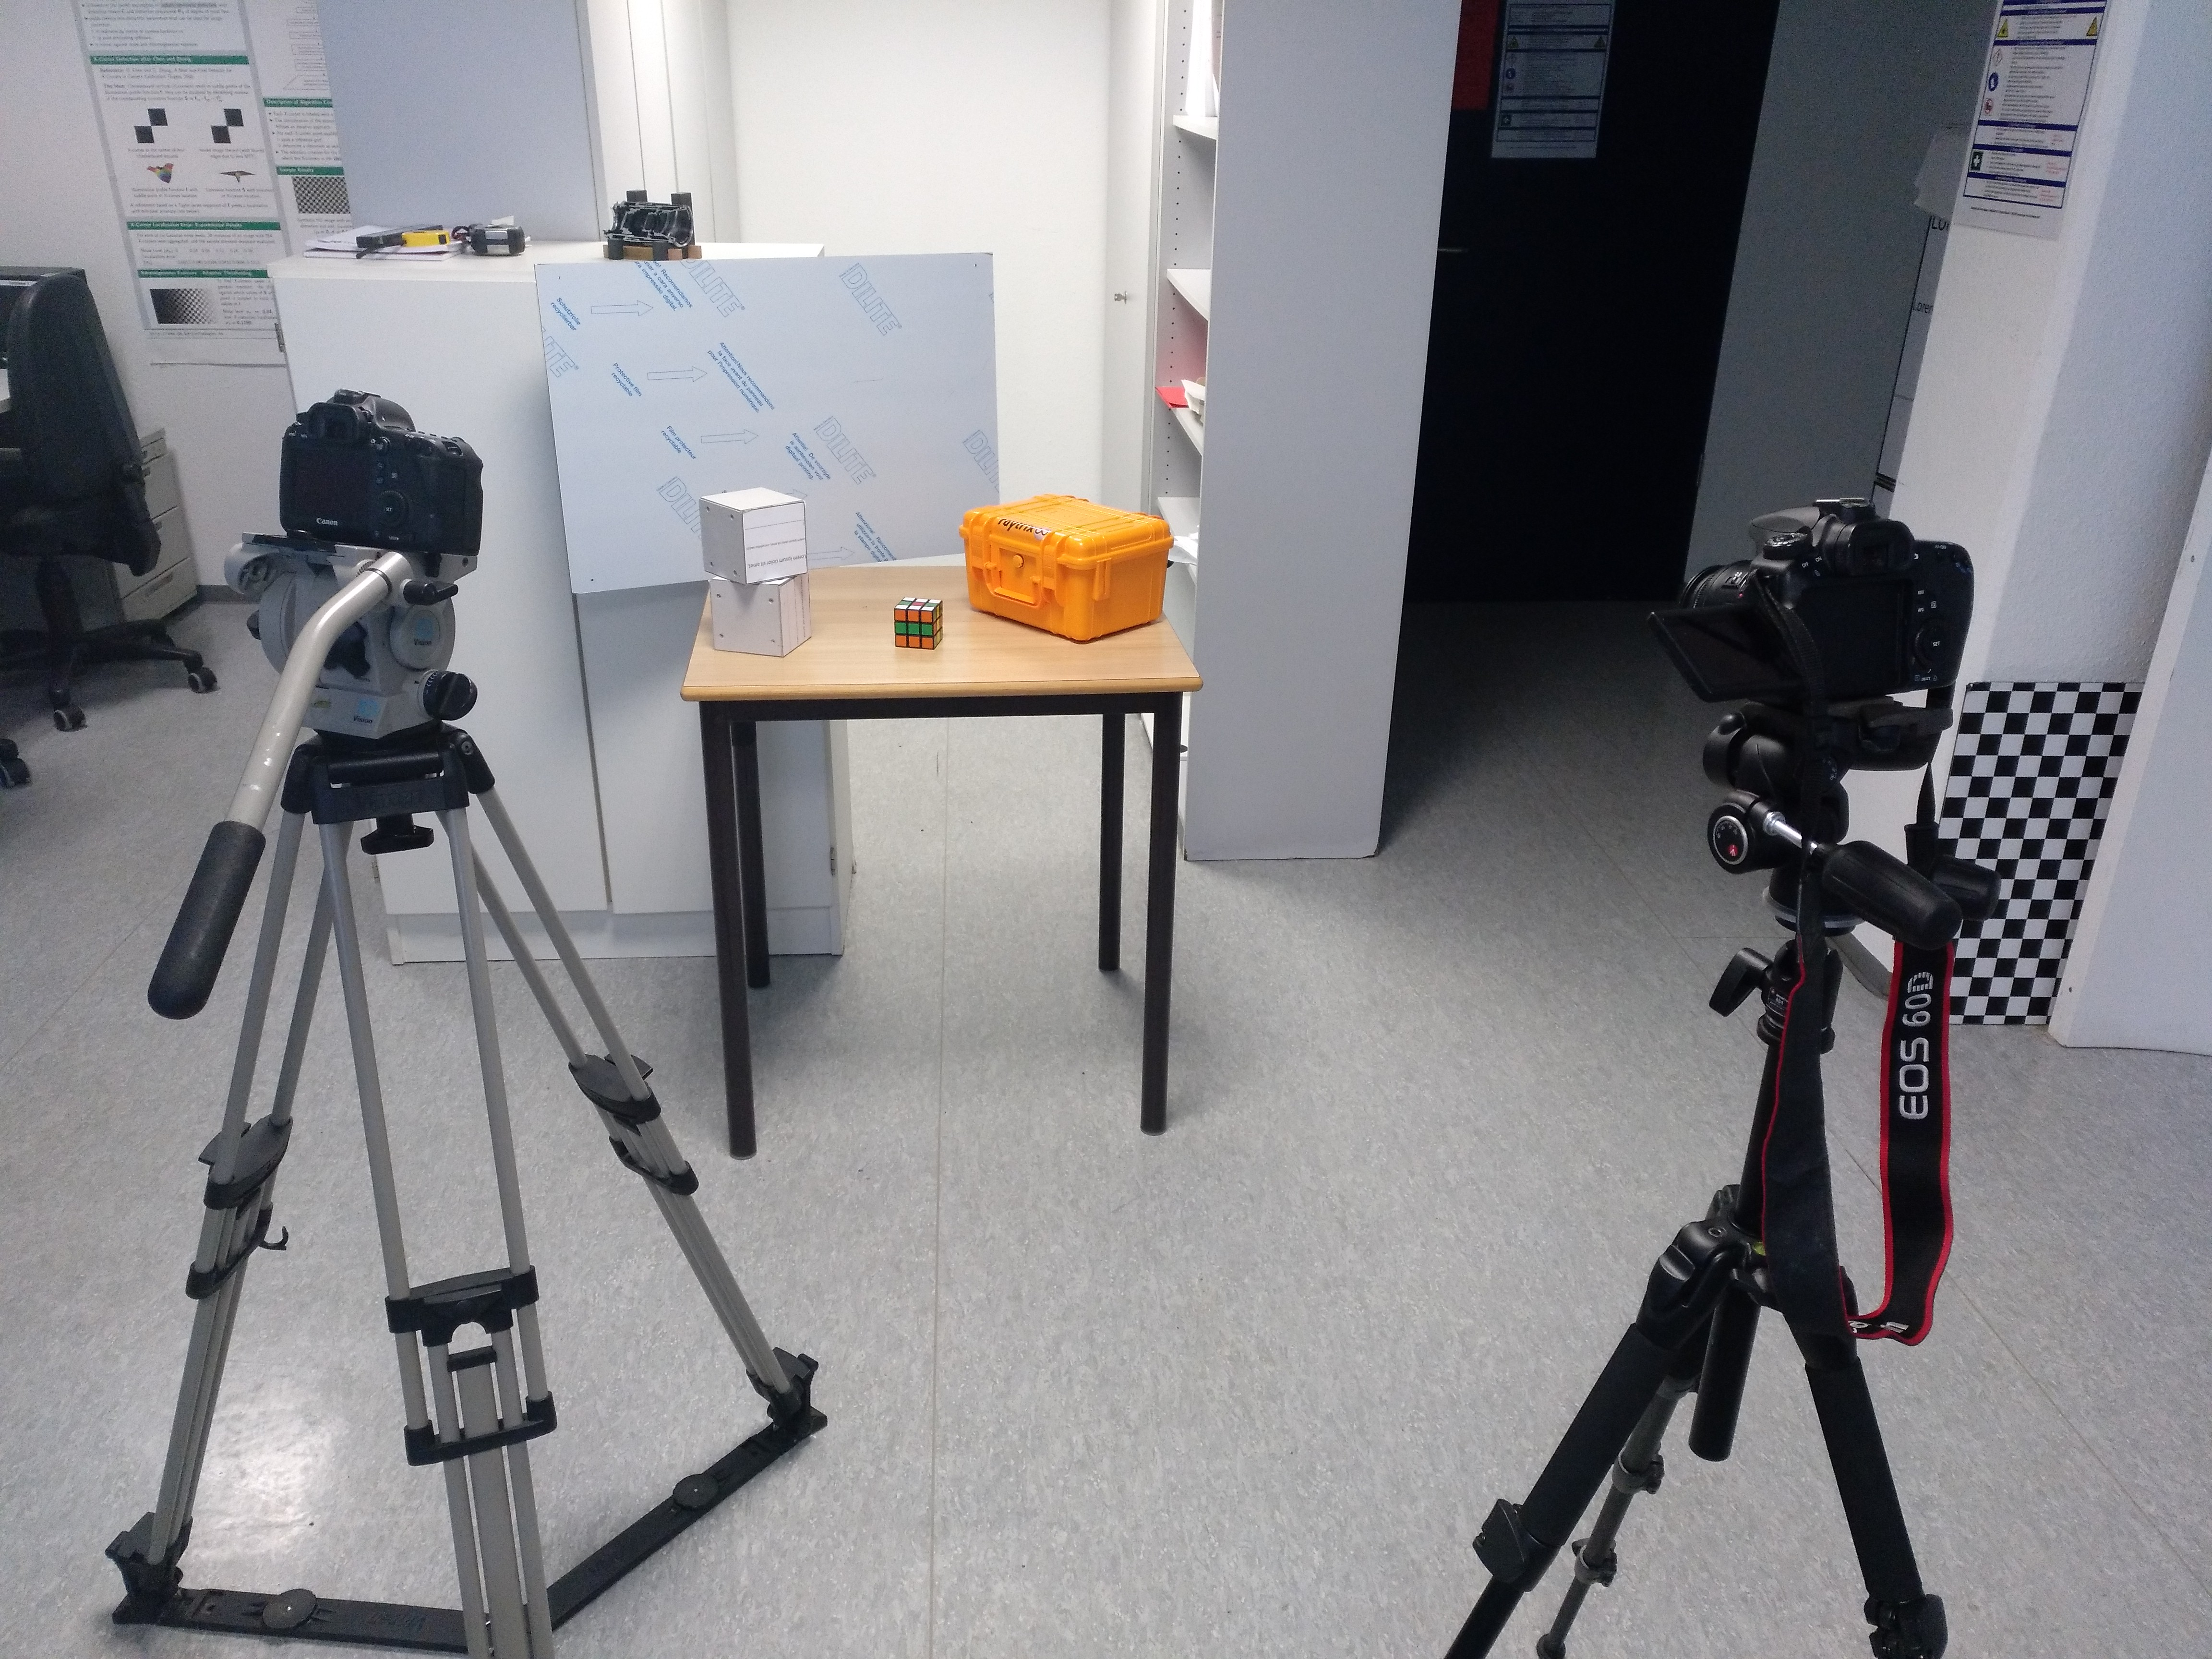
\includegraphics[width=.7\linewidth]{images/SetUpSameResolution.jpg}
	\captionof{figure}{Szenenaufbau: Die Canon 60D befindet sich in dieser Abbildung auf der linken Seite, die Canon 60 D auf der rechten. Auf dem Tisch zwischen den Kameras ist die in den Abbildungen 6.1 und 6.1 abgebildete Szene zu sehen. Beide Kameras sind zu Szene hin gedreht.}
	\label{fig:StereoaufbauReal}
\end{minipage}\\

Die auf Abbildung \ref{fig:StereoaufbauReal} zu sehende linke Kamera wurde als Kamera eins definiert. Für Kamerakoordinatensystem $(C,\beta)$ wurde gleich dem Weltkoordinatensystem $(O,\delta)$ gesetzt. Kamera zwei mit $(C',\beta')$ befindet sich auf der Abbildung rechts. Für beide Kameras wurde in einem externen Programm die intrinsischen Kameraparameter $K$ und $K'$ bestimmt. An den Stereoaufnahmen der Szene wurde dann eine Korrespondenzanalyse gemacht.   

\section{Korrespondenzanalyse}


Für die Analyse der Korrespondierenden Punkte bei Stereoaufnahmen einer dreidimensionalen Szene wurde eine existierende Funktion von Mathematica genutzt\cite{Mathematica}. Die Funktion basiert auf dem Prinzip eines SURF-Algoruthmus. SURF ist die Kurzform für  \textit{Speeded Up Robust Features} und ist ein Rotations- und Skaleninvarianter Punkte Detektor und Deskriptor\cite{SURF,SIFTSURF}. Es werden Punkte an markanten Stellen in beiden Bildern detektiert, wie beispielsweise Eckpunkte oder Kanten. Die Umgebung eines jeden gefundenen Punktes wird durch einen Merkmalsvektor, dem Deskriptor, beschrieben. Die Deskriptoren beider Bilder werden abgeglichen und gleiche Punkte werden als korrespondierende Punkte gekennzeichnet\cite{SURF,SIFTSURF}. Die Abbildungen \ref{fig:SurfLinks} und \ref{fig:SurfRechts} zeigen die Ergebnisse nach der Anwendung des SURF-Algorithmus auf das Stereobildpaar. Eine eigens implementierte alternative für die Korrespondenzanalyse zwischen Stereoaufnahmen eines zweidimensionalen Schachbretts wird in Kapitel \ref{sec:schachbrettAlg} vorgestellt.  


%	\minipage{0.48\textwidth}
%	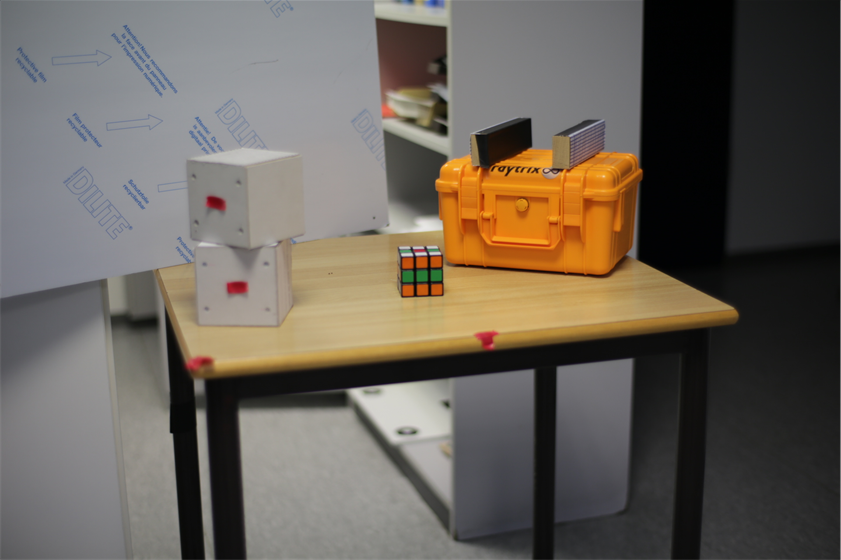
\includegraphics[width=\linewidth]{images/Points3DSceneLeft.png}
%	\caption{Aufnahme der Canon 6D von links}
%	\label{fig:awesome_image1}
%	\endminipage\hfill
%	\minipage{0.48\textwidth}
%	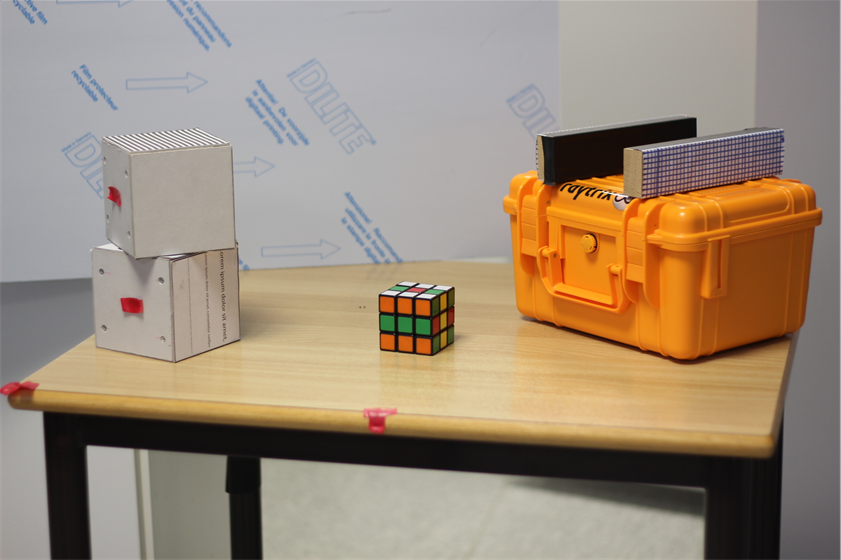
\includegraphics[width=\linewidth]{images/Points3DSceneRight.png}
%	\caption{Aufnahme der Canon 60D von rechts}
%	\label{fig:awesome_image2}
%	\endminipage\hfill
%\end{figure}
\begin{figure}[!htb]
	\minipage{0.48\textwidth}
	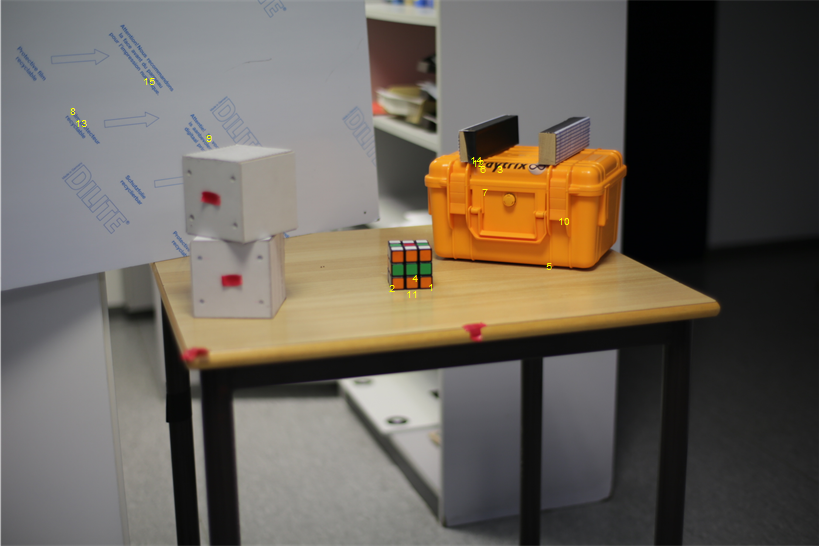
\includegraphics[width=\linewidth]{images/PointsDetectedLeft.png}
	\caption{a}
	\label{fig:SurfRechts}
	\endminipage\hfill
	\minipage{0.48\textwidth}
	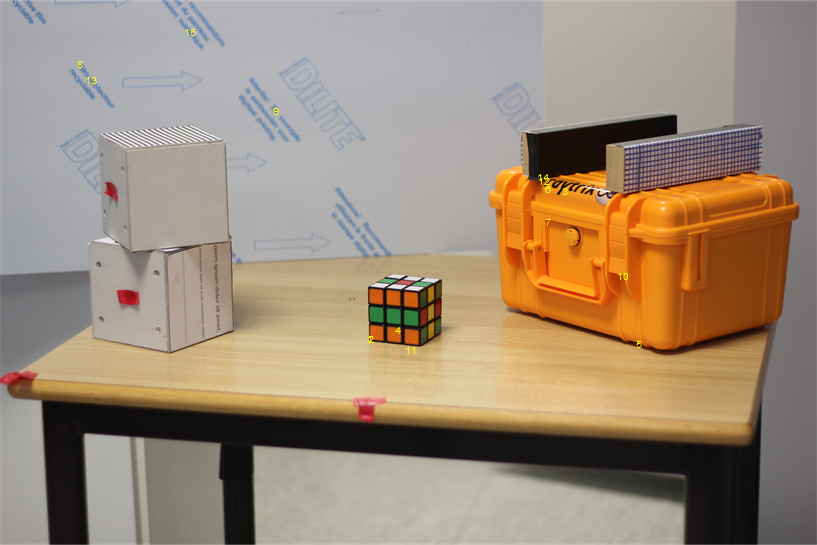
\includegraphics[width=\linewidth]{images/PointsDetectedRight.png}
	\caption{b}
	\label{fig:SurfLinks}
	\endminipage\hfill
%	\caption{Die mit dem \textit{SURF}-Algorithmus gefundenen Punkte sind mit den gelben Ziffern im Bild gekennzeichnet. Abbildung a zeigt das Bild von $C$, die Abbildung b zeigt das Bild von $C'$}
\end{figure}
\pagebreak

Die mit dem \textit{SURF}-Algorithmus gefundenen Punkte sind mit den gelben Ziffern im Bild gekennzeichnet. Abbildung a zeigt das Bild von $C$, die Abbildung b zeigt das Bild von $C'$.\\

Die Detektion von korrespondierenden Punkten mit Detektionsalgorithmen, wie Beispielsweise dem angewendeten SURF-Algorithmus, können immer Fehler und Abweichungen mit sich bringen. Die Ursprünge der Fehler können sowohl durch den Algorithmus als auch durch Fehler, wie Bildrauschen, in den Aufnahmen selbst. Diese Fehler wirken sich sowohl auf die bestimmung der Abildungsvorschriften $F$ und $E$ aus und somit auch auf die Genauigkeit der Szenenrekonstruktion\cite{HZ}. Im folgenden werden sowohl die Fehler als auch Methoden für deren Minimierung vorgestellt.

\section{Normierter acht-Punkt-Algorithmus}

Trotz das der acht-Punkt-Algorithmus eine einfache Methode zur Bestimmung der Fundamentalmatrix bietet, ist er sehr unstabil sobald Fehler wie Ungenauigkeiten in Punktekorrespondenzen oder Rauschen in Bilder auftreten\cite{HZ,Brooks}.\\

Der Fehler lässt sich anhand der Kondition der Koeffizientenmatrix $A$ genauer beschreiben. Als Kondition wird die Abhängigkeit der Lösung eines Problems von der Störung der Eingangsdaten beschrieben\cite{HZ8,ConditionNumber,Manocha}. Die Kondition lässt sich durch Bestimmung des kleinsten Eigenvektors der Matrixmultiplikation der Koeffizientenmatrix $A$ mit ihrer Transponierten $A^T$ herausfinden. Die Matrix $AA^T$ wird in die Matrizen $UDU^T$, wobei $U$ eine orthogonale und $D$ eine diagonale Matrix ist, zerlegt. Die Diagonaleinträge von $D$ sind in eine nicht ansteigenden Reihenfolge, woraus resultiert, dass der kleinste Singulärwert von $D$ mit der letzten Spalte von $U$ korrespondiert und somit ist die letzte Spalte von $U$ gleich dem kleinsten Eigenvektor von $AA^T$\cite{HZ8,ConditionNumber}. Wird angenommen, dass $AA^T$ eine 9 $\times$ 9- Matrix ist, so ergeben die Diagonaleinträge $d_1/d_9$ den Wert der Kondition. Je größer die Kondition ist, desto größer wirken sich schon kleinste Abweichungen der einkommenden Bilddaten, auf die aus $A$ bestimmten Matrix $F$ aus.\\

Um die Kondition möglichst klein zu halten, werden die Bildkoordinaten beider Bilder normiert. Die in Literaturquellen, vorgeschlagene Normierung beinhaltet pro Bild eine Translation und Skalierung, so dass der Schwerpunkt aller Punktekorrespondenzen auf einem Bild im Ursprung des Sensorkoordinatensystems liegt und der durchschnittliche Abstand der Punkte zum Ursprung $\sqrt{2}$ beträgt\cite{HZ,Ferid,Brooks}.\\

Für die Normierung wird pro Bild eine Transformationsmatrix $T$ und $T'$ definiert. Die Matrizen beinhalten sowohl eine Skalierung als auch eine Translation. Die Bestimmung der Matrix $T$ wird hier aufgezeigt. Zuerst wird der Schwerpunkt $s$ mit $s=\begin{pmatrix}
s_x\\
s_y
\end{pmatrix}$ der Punktemenge $p_n$ mit $p_n = \begin{pmatrix}
p_{nx}\\
p_{ny}
\end{pmatrix}$ berechnet, indem der Mittelwert aller Punkte $p_n$ berechnet wird.

\begin{gather}
	\begin{pmatrix}
		s_x\\
		s_y
	\end{pmatrix} = \frac{1}{n} \sum_{i = 1}^{n} \begin{pmatrix}
	p_ix\\
	p_iy
\end{pmatrix}
\end{gather}

Danach wird $s$ in den Ursprung verschoben. Die Punkte $x_n$ werden um den Wert von $s$ verschoben $x'_n = x_n - s$. Der Mittelwert aus den um $s$ verschobenen Punkten $x'_n$ ergibt den neuen Schwerpunkt $s_0$ im Koordinatenursprung. Als nächstes wird die Distanz jedes Punktes von $x'_n$ zu $s_0$ berechnet und der Mittelwert aller Distanzen, hier mit $d$ bezeichnet, berechnet. Die Matrix $T$ und $T'$ haben dann die folgende Form:

\begin{gather}
	T = \begin{pmatrix}
		\frac{\sqrt{2}}{d}&0&-s_x\\
		0&\frac{\sqrt{2}}{d}&-s_y\\
		0&0&1
	\end{pmatrix}\\
	T' = \begin{pmatrix}
	\frac{\sqrt{2}}{d'}&0&-s'_x\\
	0&\frac{\sqrt{2}}{d'}&-s'_y\\
	0&0&1
\end{pmatrix}
\end{gather}

Die originalen Bildpunkte des Stereobildpaares, werden mit den Matrizen $T$ und $T'$ verrechnet. Mit den Normierten Bildkoordinaten wird dann wieder nach dem in Kapitel \ref{sec:8pointAlg} beschriebenen acht-Punkte-Algorithmus eine Fundamentalmatrix $\hat{F}$ bestimmt\cite{HZ,HZ8,Ferid,Brooks}. Nachdem $\hat{F}$ aus den normierten Koordinaten bestimmt wurde, wird sie mit $T$ und $T'$ wieder denormalisiert.

\begin{gather}
	F = T'^T\hat{F}T
\end{gather}

%Nachdem die korrespondierenden Punkte in den Bilder gefunden wurden, wird nun der Arbeitsprozess wie in den Abbildungen ??? und ??? in der Einleitung und wie bereits aus dem Minimalbespiel bekannt, weiterverfolgt. In den einzelnen Schritten müssen jedoch ein paar Änderungen vorgenommen werde, um die durch die ungenauen Bilddaten entstehenden Fehler im Verlauf des Arbeitsprozesses zu minimieren. 

%
%Als erstes erfolgt die Schätzung der Fundamentalmatrix. Für die Schätzung wurde eine leicht abgeänderte Form des \textit{eight-point-algorithms} namens \textit{normalized-eight-point-algorithm} angewandt\cite{HZ,HZ8,Ferid}.\\ 

%
%Zur Durchführung des \textit{normalized-eight-point-algorithm} wird eine vorherige Normierung der eingehenden Bildpunkte pro Bild verlangt. Diese sollen so normiert werde, dass ihr durchschnittlicher Abstand zu ihrem den Koordiantenursprung verschobenenen Schwerpunktes $\sqrt{2}$ beträgt\cite{HZ,HZ8,Ferid}. \\

%Zu aller erst werden die jeweiligen Schwerpunkte der Punkte in den einzelnen Bildern gesucht und dieser dann in den jeweiligen Sensorkoordinatenursprung verschoben. Die Bildpunkte werden unter Beibehaltung ihres momentanen Abstandes zum Schwerpunkt mit verschoben. Danach werden die Anbständer der Bildpunkten zum Schwerpunkt so skaliert, dass der Durchschnittsabstand der Punkte zu Schwerpunkt $\sqrt{2}$ beträgt. Die so skalierten Bildpunkte befinden sich nun in einem deutlich kleineren Zahlenbereich von circa $-1$ bis $1$\cite{HZ,HZ8,Ferid,Brooks}. Die transformation der Bilddpunkte für beide Bilder wird jeweils einer Matrix $T$ und $T'$ vollzogen\cite{HZ,Brooks}.

%
% Diese Matrix ist wichtig, um nach dem schätzen einer auf den normalisierten Koordinaten basierten Fundamentalmatrix $\hat{F}$ wieder eine denormalisierte $F$ zu generieren. Die Normierung der Bildkoordinaten ist wichtig, um die Auswirkung der Bildfehler auf das Endergebnis zu minimieren.  Die Entscheidung den normalized-8-Point-Algorithm  zu benutzen fiel als festgestellt wurde, dass ohne vorherige Normalisierung der ausgelesenen Punkte es zu größeren Fehlern in den weiteren Berechnungen kam. \\
%
%
%Zur Erklärung dieser Fehler kann zum einen die \textit{Condition-Number} betrachten. Als \textit{Condition Number}, Kondition im deutschen, wird die Abhängigkeit der Lösung eines Problems von der Störung der Eingangsdaten beschrieben. 

%Die Kondition lässt sich durch Bestimmung des kleinsten Eigenvektors der Matrixmultiplikation der Koeffizientenmatrix $A$ mit ihrer Transponierten $A^T$ herausfinden. Die Matrix $AA^T$ wird in die Matrizen $UDU^T$, wobei $U$ eine orthogonale und $D$ eine diagonale Matrix ist, zerlegt. Die diagonaleinträge von $D$ sind in einen nicht ansteigenden Reihenfolge, woraus resultiert, dass der kleinste Singulärwert von $D$ mit der letzten Spalte von $U$ korrespondiert und somit ist die letzte Spalte von $U$ gleich dem kleinsten Eigenvektor von $AAt$\cite{HZ8}. Wird angenommen, dass $AA^T$ eine 9 $\times$ 9- Matrix ist, so ergeben die Einträge $d_1/d_9$ die gesuchte \textit{Condition Number}. je größer die \textit{Condition-Number} ist, desto größer wirken sich auch kleinste Abweichungen, wie Bildrauschen, auf die Resultate aus.

%Da sich die original Bildkoordinaten in diesem Beispiel in einem Zahlenbereich von 0 bis 5478 befinden, sind auch die Werte innerhalb der Koeffizientenmatrix in einem sehr großen Zahlenbereich, was zu Folge hat, das schon kleinste Abweichungen in den Bilddaten, große Auswirkungen auf die daraus resultierende Fundamentalmatrix haben kann, in Bezug darauf, dass die Werte der Einträge innerhalb von $F$, sehr große Ungleichgewichte aufweisen. Anders im Fall von Normierten Koordinaten, deren Zahlen sich in einem Bereich zwischen circa -1 und 1 befinden.  
%
%\begin{gather}
%	F = \begin{pmatrix}
%		10^{-4}&10^{-4}&10^{-2}\\
%	10^{-4}	&10^{-4}&10^{-2}\\
%		10^{-2}&10^{-2}&1
%	\end{pmatrix}\\
%	F = \begin{pmatrix}
%	-10^{-9}&10^{-6}&-10^{-4}\\
%	-10^{-7}&10^{-4}&10^{-3}\\
%	10^{-4}&-10^{-3}&-10^{-2}
%\end{pmatrix}
%\end{gather}
%
%Gleichung 6.2 zeigt schematisch was unter einer Gleichgewichtigen Fundamentalmatrix zu verstehen ist, welche bei einer sehr gereingen \textit{Condition-number} resultieren kann. Gleichung 6.3 wiederum zeigt schematisch das Resultat einer Ungleichgewichteten Fundamentalmatrix, dessen \textit{Condition-Number} sehr groß ausfällt\cite{HZ8}. 

%
%Durch normieren der Bildkoordinaten, kann die \textit{Condition-Number} kleiner und damit einhergehend die entstehenden Fehler minimiert werden.\\
%
%
%Nachdem die Fundamentalmatrix aus den normierten Koordinaten geschätzt wurde, wird sie anschließend mit den beiden aufgestellten Matrizen $T$
%und $T'$ wieder denormalisiert, so dass sie wieder als $epipolar-contraint$ zwischen die original Koordinaten geschallten werden kann. \\
%
%Für normierte Koordinaten $\hat{m}$ und $\hat{m}'$ gilt $\hat{m}'^T \cdot \hat{F} \cdot \hat{m} = 0$ und für die ursprünglichen Bildkoordinaten gilt, dass $m'^T \cdot T'^T \cdot \hat{F} \cdot T\cdot m = 0$ und somit wieder $m'^T \cdot F\cdot m = 0$ \cite{HZ,HZ8,Ferid}.\\

%Die Normierung der Koordinaten für die Verwendung des \textit{eight-point-algorithms} darf auf keinen Fall mit der Normierung der Koordinaten für die essentielle Matrix $E$ verglichen werden. Die Normierung der Koordinaten für die Schätzung von $F$, soll die Auswirkungen von Fehler auf die Resultate minimieren, während die Normierung der Koordinaten durch deren Verrechnung mit den Kameramatrizen $K$ und $K'$ dafür sorgt, dass daraus normierte Bildkoordinaten entstehen, dess Koordinatenursprung nicht mehr in einer Bildecke sondern in der Bildmitte sich befindet\cite{HZ}. 
%
%Um zurück zum Arbeitsprozess zu kommen, sind die Koordinaten normiert, so wird der im Kapitel \nameref{sec:einleitung} aufgezeigte Verfahren zur Schätzung der Fundamentalmatrix gleichermaßen wie in den Gleichungen 4.29 bis 4.34 aufgebaut.

%Durch die möglichen Ungenauigkeiten wie Bildrauschen oder dem detektieren der korrespondierenden Punkte, ist der Rang der aufgestellten Koeffizientenmatrix $A$ in den meisten Fällen größer als acht, was bedeutet, dass hier nicht einfach der Kern mit $A\cdot f = 0$ gesucht werden kann, um eine Lösung zu finden. (Einfach auf Kapitel verweisen sollte jetzt langsam klar sein)
%
%Im Falle eines höhren Ranges als 8 muss ein Verfahren, ähnlich wie dem, welches angewandt wurde um überbestimmte Systeme zu Lösen um eine Homographiematrix zu erhalten. Es wird also derjenige Vektor für $f$ gesucht, welcher $||A\cdot f||$ minimiert. Hierzu wird eine Singulärwertszerlegung von $A$ in $A  = UDV^T$ durchgeführt. die Lösung für $f$, welche $||A\cdot f||$ minimiert ist dann diejenige Spalte von $V^T$, welche mit dem kleinsten Singulärwert von $D$ korrespondiert. Da die Singulärwerte eine absteigende Reihenfolge besitzen, bildet die letzte Spalte von $V^T$ den Vektor $f$\cite{HZ}.\\


\subsection{Singularität der Fundamentalmatrix}
\label{sec:realFun}

Eine Fundamentalmatrix ist im optimalen Fall eine singuläre Matrix mit Rang 2. Die singularität der Fundamentalmatrix sorgt zum einen dafür das ihr rechter und linker Kern jeweils den Epipol des jeweilgen Bildes ergibt und die Epipolarlinien auch alle durch eben diese Epipole verlaufen\cite{HZ}. Durch Ungenauigkeiten in korrespondierenden Bildpunkten kann es dazu kommen, dass die aus dem normierten-acht-Punkt-Algorithmus bestimmte Fundamentalmatrix $\hat{F}$ in ihrem Rang steigt und ist somit keine singuläre Matrix mehr ist. Sollte dies der Fall sein, so ergeben der linke und der Rechte Kern von $F$ keine eindeutigen Lösungen mehr für $e$ und $e'$ und die Epipolarlinien in beiden Bildern gehen dem enstprechend auch nicht mehr durch genau einen Punkt, wie man in den Abbildungen \ref{fig:NoEpipoleWithF1} und \ref{fig:NoEpipoleWithF2} erkennen kann. Die Abbildungen bilden Epipolarlinien aus dem Stereobildpaar \ref{fig:SurfRechts} und \ref{fig:SurfLinks} ab.\\

\pagebreak
%
%irgendwie sagen dass es durch verunreinigte daten zu fehlern im constraint kommt und die Fundamentalmatrix im Rang steigt.
%
%Die Fundamentalmatrix ist eine singuläre-Matrix und ist somit eine Matrix von Rang zwei. Di
%
%wird die Fundamentalmatrix durch eine Singulärwertszerlung von $A$ geschätzt, ist die Chance sehr hoch, dass das Ergebnis für $\hat{F}$ eine Matrix von Rang 3 ist. Sollte dies der Fall sein gehen die Epipolarlinien der Bilder nicht mehr durch genau einen Punkt, wie man in den Abbildungen 6.5 und 6.6 erkennen kann. Diese bilden Epipolarlinien in einem Stereobildpaar ab.\\

\begin{figure}[!htb]
	\minipage{0.48\textwidth}
	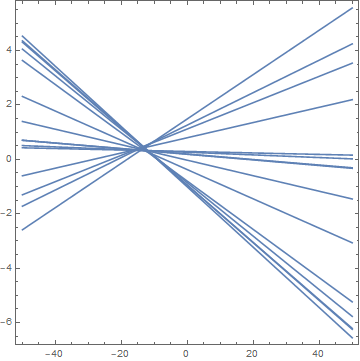
\includegraphics[width=\linewidth]{images/L_F_no_Constraint.png}
	\caption{Epipolarlinien ohne \textit{Epipolar-constraint} im Bild der Canon 6D}
	\label{fig:NoEpipoleWithF1}
	\endminipage\hfill
	\minipage{0.48\textwidth}
	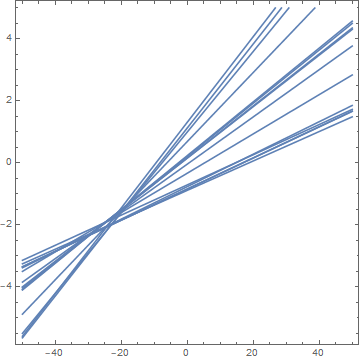
\includegraphics[width=\linewidth]{images/LPrime_PC2_F_no_Constraint.png}
	\caption{Epipolarlinien ohne \textit{Epipolar-constraint} im Bild der Canon 60D}
	\label{fig:NoEpipoleWithF2}
	\endminipage\hfill
	%	\caption{Die mit dem \textit{SURF}-Algorithmus gefundenen Punkte sind mit den gelben Ziffern im Bild gekennzeichnet}
\end{figure}

%Um eine gültige Fundamentalmatrix für den weiteren Arbeitsprozess zu generieren, kommt hier ein sogenannter \textit{singularity constraint} zum Einsatz.

Um mit dem Algorithmus weiter verfahren zu können, muss die Singularität in $\hat{F}$ erzwungen werden\cite{HZ}. Hierfür wir eine Singulärwertszerlegung an $\hat{F}$ durchgeführt, so dass $\hat{F}$ in $\hat{F} = U\Sigma V^T$ zerlegt wird. $\Sigma$ beinhaltet in einer Diagonalmatrix die Singulärwerte $D = \text{diag}(r,s,t)$. Die Diagonaleinträge erfüllen die Bedingung, dass $r \leq s \leq t $ gilt. Damit $\hat{F}$ zu einer singulären Matrix wird, muss für die Diagonaleinträge gelten, dass  $\Sigma = \text{diag}(r,s,0)$ ist. Dem entsprechend wird der letzte Eintrag $t$ auf $t = 0$ gesetzt und eine modifizierte Fundamentalmatrix mit $\bar{F} = U\text{diag}(r,s,0)V^T$ wieder zusammengesetzt. Die resultierende Fundamentalmatrix $\bar{F}$ besitzt jetzt einen Rang 2 und ist somit singulär\cite{HZ}. $\bar{F}$ ist somit, laut Frobenius Norm, die nächste zu $F$ liegende singuläre Matrix\cite{HZ}\\

Werden aus $\bar{F}$ der rechte und linke Kern bestimmt, so ergeben sich eindeutige Lösungen für $e$ und $e'$ und die Epipolarlinien $l$ und $l'$ verlaufen jeweils durch ihre entsprechenden Epipole\cite{HZ}. Die Abbildungen \ref{fig:EpipoleWithF1} und \ref{fig:EpipoleWithF2} zeigen die Auswirkung der erzwungenen Singularität von $F$ auf dem Stereobildpaar \ref{fig:SurfRechts} und \ref{fig:SurfLinks}. Die Abbildungen \ref{fig:EpipoleWithF1Denorm} und \ref{fig:EpipoleWithF2Denorm} die selben Epipolarlinien nur ist $\bar{F}$ mit $T$ und $T'$ denormalisiert worden.\\

% Zu aller erst wird eine Singulärwertszerlegung an $F$ durchgeführt, so dass $\hat{F}$ in $\hat{F} = UDV^T$ zerlegt wird. $D$ beinhaltet in einer diagonalen Matrix die Singulärwerte $D = \text{diag}(r,s,t)$, welche die Bedingung $r \leq s \leq t $ erfüllen. 
% 
% Um nun den \textit{singularity-constraint} in $\hat{F}$ zu erzwingen, wird der letzte Singulärwert $t = 0$ gesetzt, so dass am Ende dasteht $D = \text{diag}(r,s,0)$. Danach werden die Matrizen $UDV^T$, wobei $D$ nun die modifizierten Singulärwerte beinhaltet, wieder zu $\hat{F}$ multipliziert. Die jetzt resultierende Fundamentalmatrix $\hat{F}$ besitzt den Rang 2. Der rechte und linke Kern ergeben wieder die Epipole und die Epipolarlinien verlaufen wieder durch eben diese Epipole. Die Abbildungen 6.7 und 6.8 zeigen die selben Epipolarlinien wie in 6.5 und 6.6 nachdem der \textit{singularity-constraint} in $\hat{F}$ erzwungen wurde. Die somit entstandene Matrix $\hat{F}$, ist die laut Frobenius norm, nächste zum ursprünglichen $\hat{F}$\cite{HZ}.

%Jetzt erst erfolgt die zuvor erwähnte denormierung von $\hat{F}$ durch $T$ und $T'$. Die Abbildungen 6.9 und 6.10 zeigen die Epipolarlinien im Originalbild mit denormierten Koordinaten.



\begin{figure}[!htb]
	\minipage{0.48\textwidth}
	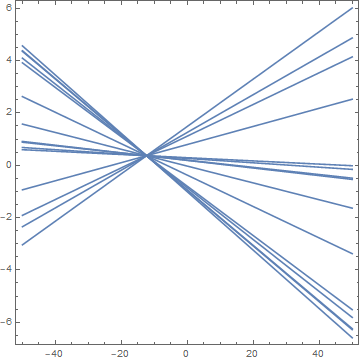
\includegraphics[width=\linewidth]{images/L_PC1_F_Constraint.png}
	\caption{Die Abbildung zeigt, dass die Epipolarlinien auf der Aufnahme von $C$, nach dem Erzwingen der singularität in der normierten $\hat{F}$, alle durch einen Epipol verlaufen}
	\label{fig:EpipoleWithF1}
	\endminipage\hfill
	\minipage{0.48\textwidth}
	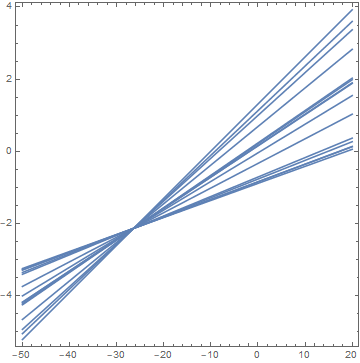
\includegraphics[width=\linewidth]{images/LPrime_PC2_F_Constraint.png}
	\caption{Die Abbildung zeigt, dass die Epipolarlinien auf der Aufnahme von $C'$, nach dem Erzwingen der singularität in der normierten $\hat{F}$, alle durch einen Epipol verlaufen}
	\label{fig:EpipoleWithF2}
	\endminipage\hfill
	%	\caption{Die mit dem \textit{SURF}-Algorithmus gefundenen Punkte sind mit den gelben Ziffern im Bild gekennzeichnet}
\end{figure}

\begin{figure}[!htb]
	\minipage{0.48\textwidth}
	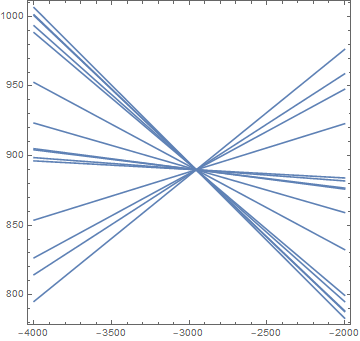
\includegraphics[width=\linewidth]{images/L_PC1_F_Constraint_denormalized.png}
	\caption{Die Abbildung zeigt die Epipolarlinien in $C$ nachdem die Fundamentalmatrix $\bar{F}$ mit $F = T'\bar{F}T$ denormalisiert wurde}
	\label{fig:EpipoleWithF1Denorm}
	\endminipage\hfill
	\minipage{0.48\textwidth}
	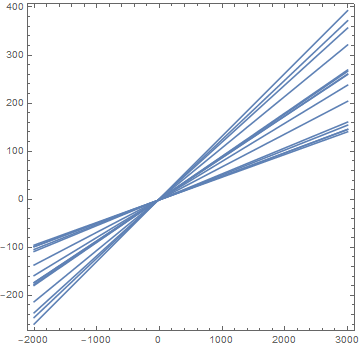
\includegraphics[width=\linewidth]{images/LPrime_PC2_F_Constraint_denormalized.png}
	\caption{Die Abbildung zeigt die Epipolarlinien in $C'$ nachdem die Fundamentalmatrix $\bar{F}$ mit $F = T'\bar{F}T$ denormalisiert wurde}
	\label{fig:EpipoleWithF2Denorm}
	\endminipage\hfill
	%	\caption{Die mit dem \textit{SURF}-Algorithmus gefundenen Punkte sind mit den gelben Ziffern im Bild gekennzeichnet}
\end{figure}

\pagebreak

\subsection{Singulärwerte der essentiellen Matrix}

Die essentielle Matrix wird im entwickelten Algorithmus aus der Fundamentalmatrix $F$ bestimmt. Da zuvor der die singularität von $F$ erzwungen wurde, ist die essentielle Matrix ebenfalls eine Matrix von Rang 2\cite{HZ}. Im synthetischen Beispiel wurde gezeigt, dass für die Bestimmung der extrinsischen Kameraparameter für $E$ gelten muss, dass für ihre Singulärwerte $\Sigma = \text{diag}(1,1,0)$ gelten muss. \\

Die Ungenauigkeit der Punkte, kann auf $E$ die Auswirkung haben, dass ihre Singulärwerte die Form $\Sigma = \text{diag}(a,b,c)$ mit $c \leq b \leq a$ annehmen. Eine Matrix gilt nur dann als gültige essentielle Matrix, wenn zwei ihrer Singulärwerte gleich sind $(a = b)$ und der dritte $(c=0)$. Um diese Bedingung zu erzwingen, wird diejenige essentielle Matirix $\hat{E}$ gesucht, welche sich lauf der Frobenius Norm am nächsten an der Ursprünglichen $E$ befindet\cite{HZ,Ferid}. Diese Matrix lässt sich aus $E = U \Sigma V^T$ bestimmen, idem eine neue essentiellem Matrix $\hat{E}$ aus $\hat{E} = U \hat{\Sigma}V^T$ mit $\hat{\Sigma} = \text{diag}(\frac{a+b}{2},\frac{a+b}{2},0)$\cite{HZ}.\\

Nach erzwingen der Bedingung $\hat{E} = U \hat{\Sigma}V^T$ mit $\hat{\Sigma} = \text{diag}(\frac{a+b}{2},\frac{a+b}{2},0)$, ist $E$ wieder eine gültige essentielle Matrix und der Algorithmus kann mit der Bestimmung der extrinsischen Kameraparameter, wie in Kapitel \ref{sec:minimal} gezeigt, fortfahren.

% wenn sie durch eine Singulärwertszerlegung in $E = U\Sigma V^T$ zerlegt wird, f

%Die essentielle Matrix $E$ kann wenn sie über den \textit{eight-point-algorithm} ermittelt wird, auch eine Rang 3 Matrix anstelle einer Rang 2 Matrix sein. Eine essentielle Matrix wird darüber definiert, dass sie eine Matrix mit Rang 2 ist und ihre Singulärwerte in $D$ von $E = UDV^T$ die Eigenschaft besitzen, dass $ D = diag(a,b,c)$ mit $a=b$ und $c=0$. Sind die Singulärwerte nicht in der gezeigten Form vorhanden und $E$ hat den Rang 3, so ist sie keine gültige essenetielle Matrix\cite{HZ}. Im implementierten Algorithmus, welcher in dieser Arbeit vorgestellt wird, wird die essentielle Matrix über die Fundamentalmatrix $F$ und den intrinsischen Kameraparameter $K$ und $K'$ gewonnen. Da im vorherigen Schritt für die Matrix $F$ schon der \textit{singularity-constraint} erwirkt wurde, ist dadurch dass $F$ nun eine MAtrix von Ran 2 ist auch versichert, dass $E$ ebenfalls von Rang 2 ist. Jedoch bedeutet das nicht gleichzeitig, dass auch die Bedingungen für die Singulärwerte von $E$ erfüllt sind. Wird $E$ in $UDV^T$ zerlegt und die Singulärwerte in D haben beispielsweise die Form $D= diag(a,b,c)$ mit $a \geq b \geq c $, so muss auch hier die für $E$ typische singularität erzwungen werden. Die laut Frobenuis Norm nächste Matrix $E$ zur momentanen $E$ kann durch modifizieren der Singulärwerte von $D$ mit $D=diag(\frac{a+b}{2},\frac{a+b}{2},0)$ erzwungen werden\cite{HZ}. Mit der neuen essentiellen Matrix können dann genau wie im Kapitel \nameref{sec:minimal} auch wieder die vier möglichen Lösungen der externen Kameraparameter ermittelt werden. 

\section{Szenenrekonstruktion mit Sampson-Approximation}
\label{sec:sampson}

Aufgrund der Ungenauigkeit der korrespondierenden Punkte ist es nicht möglich die 3D-Objektpunkte durch einfache Rückprojektion der Bildpunkte zu rekonstruieren. Liegt der zu $m_\tau$ korrespondierende Bildpunkt $m'_{\tau'}$ nicht ganz genau auf der zu $m_\tau$ korrespondierenden Epipolarlinie, so ist der in Kapitel \ref{sec:HFE} aufgestellt \textit{Epipolar-Constraint} aus Gleichung \ref{eq:Ep6} nicht mehr erfüllt. Durch einsetzten der durch den SURF-Alggorithmus detektierten korrespondierenden Punkte $m_\tau$ und $m'_{\tau'}$ in die Gleichung 

\begin{gather}
	m'^T_{\tau'}Fm_\tau = 0
\end{gather}

kommt ein Wert $\neq 0$ heraus. Je weiter der Wert von 0 abweicht, desto ungenauer ist die korrespondenz beider Bildpunkte. Dies führt dazu, dass bei der Rückprojektion der Bildpunkte $m_\tau$ und $m'_{\tau'}$ sich die Linien nicht im Raum treffen. Die Abbildungen \ref{fig:ProblemTraingulation} und \ref{fig:lFm} veranschaulichen die Konsequenz von ungenauen Punktekorrespondenzen.
%
%ist es bei den Fehlerhaften Bildkooridinaten nicht möglich die 3D-Szenenpunkte durch eine einfache Rückprojektion der der Bildpunkte zu einem Punkt im 3D-Raum zu erhalten. 
%
%sagen dass der epipolarconstraint nicht genau erfüllt wird
%
%Grund nennen und an bilder zeigen 
%Im letzten Schritt des Arbeitsprozesses, wird nun noch die Szenen mit Hilfe eines Triangulationsverfahrens rekonstruiert. Wie bereits im Kapitel \nameref{sec:minimal} erwähnt wurde, ist es bei den Fehlerhaften Bildkooridinaten nicht möglich die 3D-Szenenpunkte durch eine einfache Rückprojektion der der Bildpunkte zu einem Punkt im 3D-Raum zu erhalten. 
%
%liegt nur einer der beiden Bildpunkte $m$ oder $m'$ nicht hundert prozentig auf der jeweilgen korrespondierenden Epipolarlinie, so liegen die rückprojizierten Strahlen windschief im Raum. Das liegt daran, dass die Bildpunkte $m$ und $m'$ nicht den \textit{Epipolar-Constraint} $m'^T F m = 0$ erfüllen. Sprich die Gleichungen $m = PM$ und $m' = P'M$ können nicht erfüllt werden, da es kein $M$ gibt, dass für beide Gleichungen mit den momentanen $m$ und $m'$ gibt. Abbildung 6.11 veranschaulicht die Rückprojektion der Kamerazentren durch zwei Fehlerhafte Bildpunkte. 

\begin{figure}[!htb]
	\minipage{0.48\textwidth}
	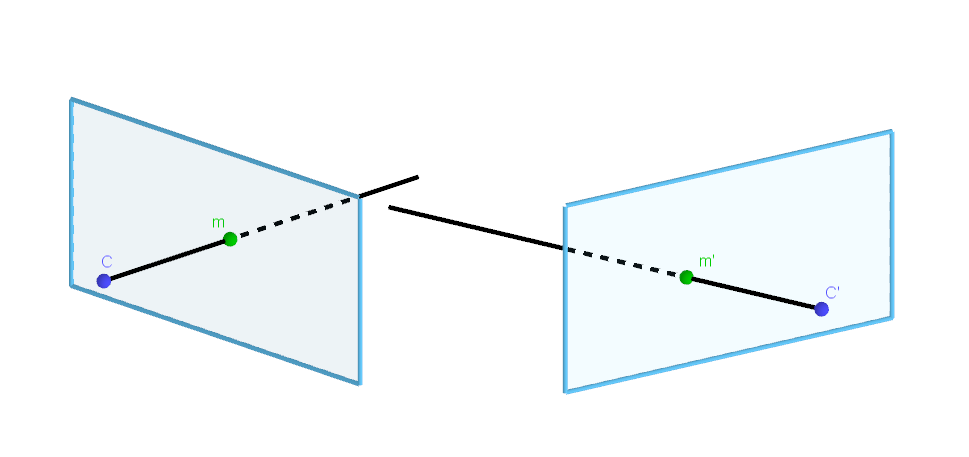
\includegraphics[width=\linewidth]{images/problemTriangulation.png}
	\caption{a)}
	\label{fig:ProblemTraingulation}
	\endminipage\hfill
	\minipage{0.5\textwidth}
	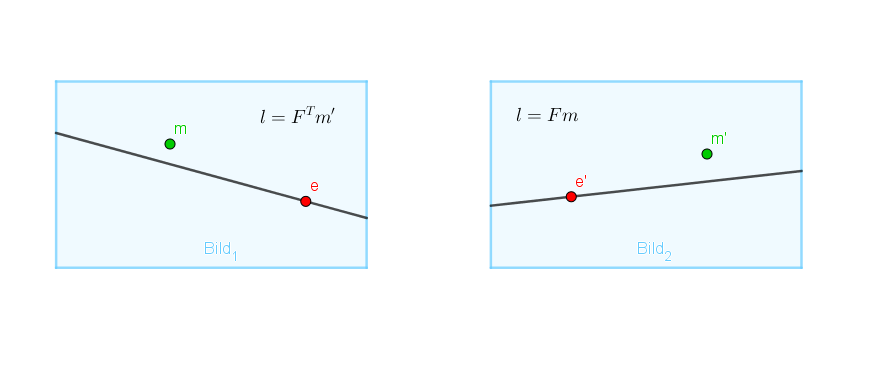
\includegraphics[width=\linewidth]{images/SampsAppx.png}
	\caption{b)}
	\label{fig:lFm}
	\endminipage\hfill
	\caption{ a) Die rückprojizierten Strahlen der ungenauen korrespondierenden Punkte $m_\tau$ und $m'_{\tau'}$ sind Windschief zueinander und treffen sich nicht in einem Punkt $M_\delta$ im Raum. b) Die korrespondierenden Bildpunkte $m_\tau$ und $m'_{\tau'}$ erfüllen nicht den \textit{Epipolar-Constraint}. Die Epipolarlinie $l' = Fm$ is die korrespondierende Epipolarlinie zu $m_\tau$ und $l = F^Tm'$ ist die korrespondierende Epipolarlinie zu $m'_{\tau}$. Da weder $m_\tau$ noch $m'_{\tau'}$ auf der Epipolarlinie zum jeweils korrespondierenden Punkt liegt, kommt es zu keinem Schnittpunkt der rückprojizierten Strahlen}
\end{figure}

Um trotz der ungenauen korrespondierenden Punkte eine Triangulation zu ermöglichen, wurde ein Verfahren voran geschaltet, welches zwei Punkte $\hat{m}_\tau$ und $\hat{m}'_{\tau'}$ sucht, die möglichst nah an den ursprünglichen Punkten $m_\tau$ und $m'_{\tau'}$ liegen und gleichzeitig den \textit{Epipolar-Constraint} $\hat{m}'^T_{\tau'}F\hat{m}_\tau = 0$ erfüllen. $\hat{m}_\tau$ und $\hat{m}'_{\tau'}$ sollen durch Minimierung einer Kostenfunktion $C$ bestimmt werden, welche die Distanz  $d$ zwischen $m_\tau$ und $\hat{m}_\tau$ und $m'_{\tau'}$ und $\hat{m}'_{\tau'}$ minimiert. Für die Minimierung wird das Verfahren der Sampson-Approximation gewählt\cite{HZ}. (Literatur zu Sampson approximation?? erklären wie??) Voraussetzung für die Triangulierung ist, dass die Projektionsmatrizen $P$ und $P'$, sowie die Fundamentalmatrix $F$ bekannt sein müssen\cite{HZ}.

\begin{gather}
	C(m,m') = d(m,\hat{m})^2 + d(m',\hat{m'})^2
\end{gather}

%Jedes Punktepaar, welches den \textit{Epipolar-Constraint} erfüllt, liegt auf einem paar korrespondierender Epipolarlinien. 

Die optimalen $\hat{m}$ und $\hat{m}'$ liegen auf den korrespondierenden Epipolarlinien $\hat{l}$ und $\hat{l}'$ am Fuße des Lots, welches von den ursprünglich projizierten Punkten $m$ und $m'$ auf die Epipolarlinien $\hat{l}$ und $\hat{l'}$ gefällt wird\cite{HZ}. 


\begin{minipage}{\linewidth}
	\centering
	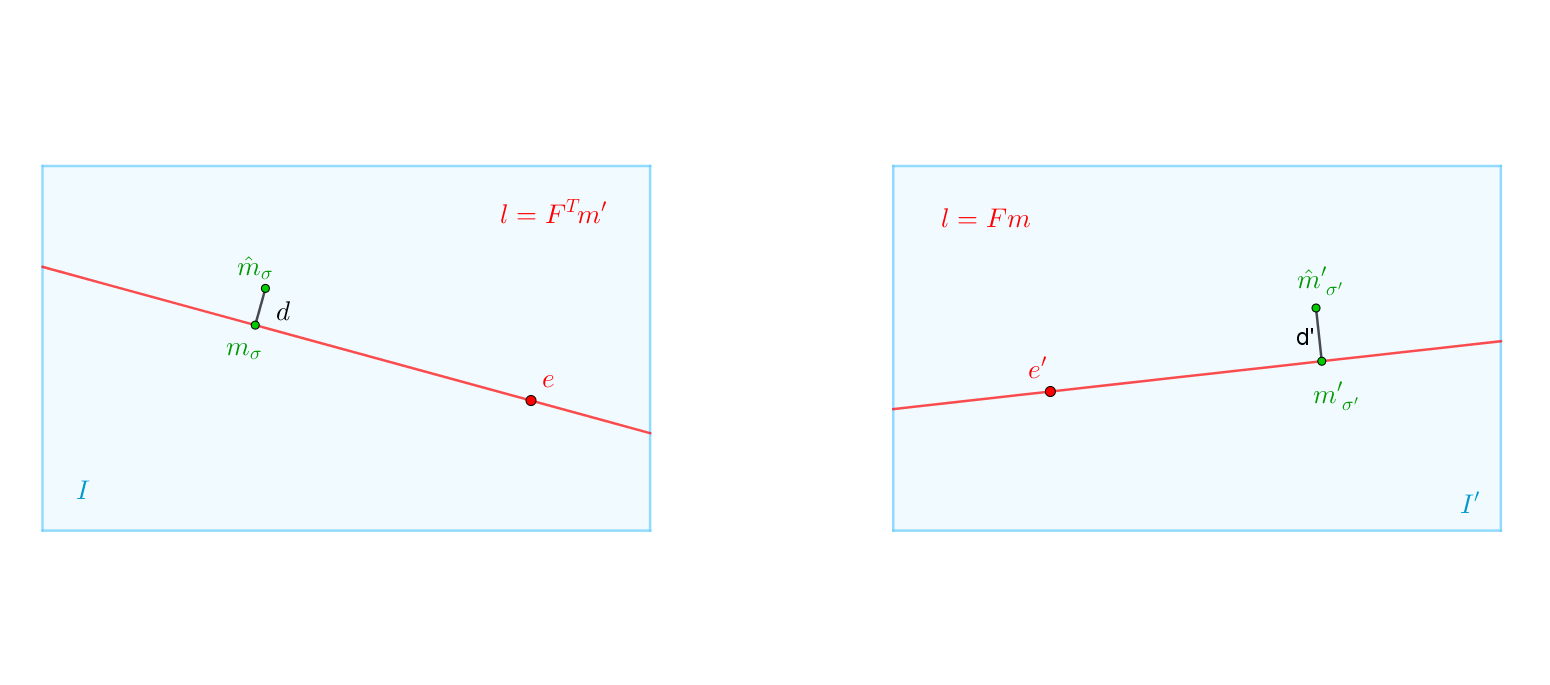
\includegraphics[width=.8\linewidth]{images/SampsAppxNewPoints.png}
	\captionof{figure}{Die Abbildung zeigt die zwei korrespondierenden Epipolarlinien $\hat{l}$ und $\hat{l'}$ mit den gesuchten Punkten $\hat{m_\tau}$ und $\hat{m'_{\tau'}}$}
\end{minipage}\\\\

Jedes andere Punktepaar auf $\hat{l}$ und $\hat{l}'$ würde den \textit{Epipolar-Constraint} erfüllen, jedoch minimieren nur $m_{\tau\bot}$ und $m'_{\tau' \bot}$ die quadratischen Distanzen $d(m_\tau,\hat{m}_\tau)^2$ und $ d(m'_{\tau'},\hat{m}'_{\tau'})^2$ in der Kostenfunktion $C$. Gesucht wird also der geringste Abstand von $m_\tau$ zu $\hat{l}$ und $m'_{\tau'}$ zu $\hat{l}'$. Die Kostenfunktion $C$ kann dem entsprechend umformuliert werden in 

\begin{gather}
	C(m,m') = d(\hat{m}_\tau,\hat{l})^2 + d(\hat{m}'_{\tau'},\hat{l}')^2
\end{gather}
.

Aus allen möglichen Epipolarlinien, welche $\hat{l}$ und $\hat{l}'$ annehmen können, wird immer der senkrechte Abstand von $m_\tau$ und $m'_{\tau'}$ zur jeweiligen Epipolarlinie berechnet. jedoch soll genau das Epipolalinienpaar gewählt werden, welches die Kostenfunktion $C$ minimal werden lässt\cite{HZ}.\\

Im ersten Schritt werden die Epipolarlinien Parametrisiert, so dass eine Linie als $\hat{l}(t)$ geschrieben werden kann. Durch die Parametrisierung der Epipolarlinien, kann die Kostenfunktion $C$ als Funktion von $t$ umformuliert werden.


\begin{gather}
	C(m_\tau,m'_{\tau'}) = d(m_\tau,\hat{l}(t))^2 + d(m',\hat{l}'(t))^2
\end{gather}


%Danach wird die Fundamentalmatrix $F$ dazu benutzt, die entsprechend korrespondierende Epiploarlinie $l'$ zu berechnen. Die Kostenfunktion $C$ kann somit als eine Funktion von $t$ definiert werden. Schlussendlich muss ein Wert für $t$ gefunden werden, welcher $C$ minimal werden lässt. 
%
%\begin{gather}
%	C(m,m') = d(m,\hat{m})^2 + d(m',\hat{m'})^2\\
%	\leadsto 
%	C(m,m') = d(m,l(t))^2 + d(m',l'(t))^2
%\end{gather}\\

Um zu verhindern dass Bildpunkte, die mit dem Epipol des anderen Bildes korrespondieren 

Bei Bildpunkten, welche mit dem Epipol des anderen Bildes korrespondieren, würde sich der rückprojizierte Objektpunkt $M_\delta$ auf der Basislinie der zwei Projektionszentren befinden. Eine Rekonstruktion des Punktes wäre nicht möglich\cite{HZ}. Um diesen Fall zu vermeiden, werden die Bildpunkte $m_\tau$ und $m'_{\tau'} $ mit jeweils einer Matrix $T$ und $T'$ in den Ursprung $(0,0,1)^T$ verschoben.

%Es kann passieren , dass ein Bildpunkt korrespondierend zum jeweiligen Epipol des anderen Bildes ist, der Rückprojizierte Punkt im 3D-Raum würde sich dann auf der Basislinie der zwei Projektionszentren befinden und es ist somit nicht möglich ihn zu rekonstruieren. Um solche Fälle zu vermeiden, wird eine Transformation der Punkte $m$ und $m'$ in den Ursprung $(0,0,1)^T$ zu verschieben.

\begin{gather}
	T = \begin{bmatrix}
	1&0&-m_{x\tau}\\
	0&1&-m_{y\tau'}\\
	0&0&1
	\end{bmatrix} \leadsto \bar{m_\tau} = T\cdot m_\tau\\
	T' = \begin{bmatrix}
	1&0&-m'_{x\tau'}\\
	0&1&-m'_{y\tau'}\\
	0&0&1
	\end{bmatrix} \leadsto 	\bar{m}'_{\tau'} = T' \cdot m'_{\tau'}
\end{gather} \\

Die Fundamentalmatrix $F$ wird ebenfalls mit $T$ und $T'$ transformiert, so dass sie an die verschobenen Punkte $\bar{m}_{\tau}$ und $\bar{m}'_{\tau'}$ angepasst ist.
%
%Die Fundamentalmatrix $F$ wird dann wieder an die neu translatierten Punkte $\bar{m}$ und $\bar{m}'$ angepasst.

\begin{gather}
	\bar{F}= T'^{-T}FT^{-1}
\end{gather}

%Als nächstes wird $F$ mit $T$ und $T$ so Transformiert, dass den \textit{Singularity-Constraint} zwischen 
Der rechte und linke Kern von $\bar{F}$ ergeben die Epipole $\bar{e}$ und $\bar{e}'$. Angenommen $f$ und $f'$ seinen genau 0, so liegen die Epipole $e = (1,0,f)^T$ und $e' = (1,0,f')^T$ im unendlichen. Ist dies der Fall so hat $\bar{F}$ für welche dann gilt, dass $\bar{F}(1,0,f)^T = (1,0,f')\bar{F}=0$ eine spezielle Form\cite{HZ}.

%Die entstehenden Epipole besitzen die Form $\hat{e}=(1,0,f)^T$ und $\hat{e'}=(1,0,f')^T$, wobei $f$ und $f'$ nahezu null sein wird. Sollten die $x$ und $y$ Werte der Epipole abweichen, so werden diese so skaliert, dass $\hat{e}^2_x + \hat{e}^2_y = 1$ ergeben, selbiges gilt auch für $\hat{e}'$.


%Des Weiteren sollen die Epipole auf die x-Achse an die Punkte $\hat{e}=(1,0,f)^T$ und $\hat{e'}=(1,0,f')^T$, wobei $f$ und $f'$ nahezu null sein werden. 

%Sind $f = 0$ und $f' = 0$, so liefen die Epipole im unendlichen. Die Epipole lassen sich durch den rechten und linken Kern der neuen $\bar{F}$ berechnen. 



\begin{gather}
	\bar{F} = \begin{pmatrix}
	ff'd&-f'c&-f'd\\
	-fb&a&b\\
	-fd&c&d\label{eq:FSampson}
	\end{pmatrix}\\
	\begin{pmatrix}
	ff'd&-f'c&-f'd\\
	-fb&a&b\\
	-fd&c&d
	\end{pmatrix} \cdot \begin{pmatrix}
	1\\0\\f
	\end{pmatrix} = 
	\begin{pmatrix}
	ff'd + (-ff'd)\\
	-fb + fb\\
	-fd +fd
	\end{pmatrix}
	= 
	\begin{pmatrix}
	0\\0\\0
	\end{pmatrix}\\
	\begin{pmatrix}
	1&0&f'
	\end{pmatrix} \cdot
	\begin{pmatrix}
	ff'd&-f'c&-f'd\\
	-fb&a&b\\
	-fd&c&d
	\end{pmatrix} =
	\begin{pmatrix}
	ff'd + (-ff'd)\\
	-f'c + f'c\\
	-f'd + f'd
	\end{pmatrix} = 
		\begin{pmatrix}
	0&0&0
	\end{pmatrix}
\end{gather}

Im Realfall sind die Werte der Epipole $e$ und $e'$ nicht so rein wie im Beispiel gezeigt. Aufgrund dessen, werden zwei Rotationsmatrizen aufgestellt, welche die Epipole $e$ und $e'$ auf $Re = (1,0,e_3) = (1,0,f)$ und $R'e' = (1,0,e'_3)=(1,0,f')$ rotiert.

\begin{gather}
	R = \begin{bmatrix}
		e_1&e_2&0\\
		-e_2&e_1&0\\
		0&0&1
	\end{bmatrix}\\
	R' = \begin{bmatrix}
	e'_1&e'_2&0\\
	-e'_2&e'_1&0\\
	0&0&1
\end{bmatrix}
\end{gather}\\

$\bar{F}$ wird dann nochmals mit $\bar{F}_{Rot} = R'FR^T$ ersetzt. Die Einträge in $\bar{F}_{Rot}$ haben nun die Form wie in Gleichung \ref{eq:FSampson}, mit $f = e_3, \, f' = e'_3, \, a = \bar{F}_{Rot,22}, \, b = \bar{F}_{Rot,23}, \, c = \bar{F}_{Rot,32}$ und $d = \bar{F}_{Rot,33}$.
Verläuft eine Epipolarlinie durch einen Punkt $(0,t,1)^T$ und dem Epipol $e = (1,0,f)^T$, wird diese Epipolarlinie mit $l(t)$ bezeichnet. Das Kreuzprodukt dieser beiden Punkte beschreibt die Epipolarlinie $l(t)$. 

\begin{gather}
\hat{l}(t)=
	\begin{pmatrix}
	0\\t\\1
	\end{pmatrix} \times
	\begin{pmatrix}
	1\\0\\f
	\end{pmatrix} = 
	\begin{pmatrix}
	tf\\1\\-t
	\end{pmatrix}
\end{gather}

Die quadratische Distanz dieser Linie zum Ursprung wird dann bezeichnet mit:


\begin{gather}
	d(\bar{m_\tau},\hat{l}(t))^2 = \frac{t^2}{1+(tf)^2} \label{eq:quadraticDistance}
\end{gather}

Für die Herleitung von Gleichung \ref{eq:quadraticDistance} wird eine Gerade zunächst in Koordinatenform Dargestellt.

\begin{gather}
	Ax+By-C = 0
\end{gather}

Die Selbe Gerade in Normalform ausgedrückt lautet:

\begin{gather}
\vec{n}\cdot (\vec{x} - \vec{p}) = 0\\
	\begin{pmatrix}
	A\\B
	\end{pmatrix}
	\cdot
	(\vec{x} - \vec{p}) = 0\label{eq:GeradengleichungSampson}
\end{gather} 

Der Abstand $\parallel \vec{v} \parallel$ eines Punktes zur Geraden \ref{eq:GeradengleichungSampson} kann folgendermaßen berechnet werden.

\begin{gather}
	\vec{v} = \frac{\vec{p} \cdot \vec{n}}{\vec{n} \cdot \vec{n}} \cdot \vec{n}
	\leadsto \frac{-C}{A^2+B^2} \cdot \begin{pmatrix}
	A\\B
	\end{pmatrix}\\
	||\vec{v}|| = \frac{|\vec{p} \cdot \vec{n}|}{||\vec{n}||^2} \cdot ||\vec{n}|| \leadsto ||\vec{v}|| = \frac{|\vec{p} \cdot \vec{n}|}{||\vec{n}||}\\
	\Rightarrow |C| = |\vec{p} \cdot \vec{n}| \\
	\Rightarrow |\sqrt{A^2+B^2}| = ||\vec{n}||\\
	||\vec{v}|| = \frac{|C|}{\sqrt{A^2+B^2}}
\end{gather}

Werden nun $A,B$ und $C$ mit den Werten der Geraden $(tf,1,-t)^T$ ersetzt, kann Gleichung \ref{eq:quadraticDistance} rekonstruiert werden.

\begin{gather}
	A = tf, \; B= 1, \; C = -t, \; \vec{v} = d\\
	d^2 = \frac{t^2}{\sqrt{((tf)^2+1^2)^2}} = \frac{t^2}{(tf)^2+ 1^2} =  \frac{t^2}{1 + (tf)^2}
\end{gather}\\

Um die zu $\hat{l}(t)$ korresponiderende Epipolarlinie $\hat{l}'(t)$ zu bestimmen, wird der Punkt $(0,t,1)^T$ und die Fundamentalmatrix $\bar{F}_{Rot}$ multipliziert.

\begin{gather}
	l'(t) = F(0,t,1)^T = (-f'(ct+d),at+b,ct+d)^T.
\end{gather}

Für die quadratische Distanz $d(m',l'(t))^2$ ergibt sich dann:

\begin{gather}
	d(\bar{m_\tau},\hat{l}(t))^2 = \frac{(ct + d)^2}{(at+b)^2+f'^2(ct+d)^2}
\end{gather} \\

Die Kostenfunktion $C$ kann jetzt in eine Funktion $s(t)$ umformuliert werden.

\begin{gather}
%	C(m,m') = d(m,\hat{m})^2 + d(m',\hat{m'})^2 \\
%	\leadsto 	C(m,m') = d(m,l(t))^2 + d(m',l'(t))^2\\
	s(t) = \frac{t^2}{1+(tf)^2} + \frac{(ct + d)^2}{(at+b)^2+f'^2(ct+d)^2}
\end{gather}

Ein Minimum für $s(t)$ kann jetzt beispielsweise durch Bestimmung der Minimas und Maximas mit $s'(t) = 0$ gefunden werden. 

\begin{gather}
	s'(t) = \frac{2t}{(1+f^2t^2)^2} - \frac{2(ad-bc)(at+b)(ct+t)}{((at+b)^2+f'^2(ct+d)^2)^2}
\end{gather}

Werden die beiden Terme in $s'(t)$ auf einen gemeinsamen Nenner gebracht und der Zähler dann gleich Null gesetzt, ergibt sich der folgende Ausdruck $g(t)$

\begin{gather}
	g(t) = t((at+b)^2+f'^2(ct+d)^2)^2-(ad-bc)(1+f^2t^2)^2(at+b)(ct+d)
\end{gather}\\

Funktion $g(t)$ ist ein Polynom vom Grad 6. Das Minimum für $s(t)$ ergibt sich aus einer der 6 möglichen Lösungen für $t$ aus $g(t)$. Für die Bestimmung des Minimums werden nur die reellen Lösungen in Betracht gezogen, die nicht-reellen Lösungen können ignoriert werden. Die reellen Lösungen für $t$ aus $g(t)$, werden dann wieder in $s(t)$ eingesetzt. Das $t$, welches durch einsetzte in $s(t)$ den kleinsten Wert ergibt, ist das gesuchte Minimum $t_{min}$. \\

Mit $t_{min}$ können die Epipolarlinien $\hat{l}(t)=(tf,1,-t)$ und $\hat{l}'(t) = F(0,t,1)^T$ durch einsetzen von $t_{min}$ berechnet werden. Danach werden die zwei neuen Punkte $\hat{m}_{\tau}$ und $\hat{m}'_{\tau'}$ auf den Epipolarlinien bestimmt. $\hat{m}_{\tau Rot}$ und $\hat{m}'_{\tau' Rot}$ sind die Punkte auf der Epipolarlinie welche dem Ursprung am nächsten sind. Der Punkt, welcher vom Ursprung aus am nächsten auf einer Linien $(\lambda, \mu,\upsilon)$ liegt, kann mit $(-\lambda \cdot \upsilon, -\mu \cdot \upsilon, \lambda^2+ \mu^2)$ berechnet werden.

\begin{gather}
	\hat{l} = (tf, 1, -t)\
	\hat{m}_{\tau Rot} = (-(tf) \cdot \upsilon , - 1 \cdot \upsilon, (tf)^2 \cdot 1^2 )\\
\end{gather}\\
 
Nachdem zu beiden Linien $\hat{l}$ und $l\hat{a}'$ der jeweils nächste Punkte $\hat{m}_{Rot}$ und $\hat{m}'_{Rot}$ vom Ursprung aus gefunden wurden, werden diese nun mit $T$, $T'$, $R$ und $R'$ wieder an ihre Ausgangsposition zurück Transformiert. 

\begin{gather}
	\hat{m} = T^{-1}R^T\hat{m}_{Rot}\\
	\hat{m}' = T'^{-1}R'^T\hat{m}'_{Rot}
\end{gather}

%Vergleicht man die Punkte $m$ und $\hat{m}$ und die Punkte $m'$ und $\hat{m'}$, so kann die minimalen Abweichungen der Punkte voneinander sehen. 


Für auf diese weise neu berechneten korrespondierneden Punkte ist der \textit{Epipolar-Constraint} \ref{eq:Ep6} erfüllt und es ist gewährleistst, dass sich ihre jeweiligen Rückprijektionen in einem Punkt im Raum treffen.\\

Für die Rückprojektion der einzelnen Bildpunkte wurde ein lineares Triangulationsverfahren gewählt\cite{HZ}. Für die Rückprojektion werden pro korrespondieredem Punktepaar zunächst die Projektionsgleichungen  $\hat{m}_\tau = P\hat{M}_\delta$ und $\hat{m}'_{\tau'}  = P'\hat{M}_\delta$ aufgestellt. Diese werden so in eine Koeffizientenmatrix $A$ eingetragen dass gilt $A\cdot x = 0$. Durch die Verwendung des Kreuzproduktes, wird die Homogene Komponente eliminiert\cite{HZ}. 

%(HIER WEITER MACHEN)
%Nachdem nun gewährleistet ist, dass sich Rückprojektion der neuen Punkte $\hat{m}_\tau$ und $\hat{m}'_{\tau'}$


%Um nun noch den Punkt $\hat{M}$ im 3D-Raum zu rekonstruieren, kann nun jegliche bekannte Methode für die Triangulierung verwendet werden. Durch die zuvorigen Rechenoperationen ist nun gewährleistet, dass sich die Gerade der Projektionszentren $C$ und $C'$ durch ihre jeweiligen Bildpunkte $\hat{m}$ und $\hat{m}'$ auf jeden Fall im Raum treffen\cite{HZ}. Für Doe Rückprojektion der Punkte $\hat{m}$ und $\hat{m}'$ zu $\hat{M}$ wurde ebefalls sich wieder auf ein Verfahren von \textit{Hartley \& Zisserman} berufen. Es handelt sich um eine lineare Triangulierungsmethode.

\begin{gather}
	\hat{m} \times (P\hat{M}) = 0\\
	\hat{m}' \times (P\hat{M}') = 0
\end{gather}

Was ausgeschrieben für $\hat{m}$ und $\hat{m}'$ zu den folgenden drei Gleichungen führt. $x \times (PX) = 0$ ergibt ausgeschrieben

\begin{gather}
x(p^{3T}X) - (p^{1T}X)=0\\
y(p^{3T}X) - (p^{2T}X)=0\\
x(p^{2T}X) - y(p^{1T}X)=0
\end{gather}
.

$p^{iT}$ bezeichnet hier jeweils die Reihen der Projektionsmatrix $P$ beziehungsweise $P'$. Zwei der drei Gleichungen sind linear unabhängig und werden in die Koeffizietenmatrix $A$ geschrieben 


% Die Matrix $A$ stellt sich, aufgrund der Tatsache, dass die Komponenten der Gleichungen 7.37 bis 7.39 linear zu $\hat{M}$ sind, wie folgt zusammen.

\begin{gather}
A = \begin{bmatrix}
xp^{3T}-p^{1T}\\
yp^{3T}-p^{2T}\\
x'p'^{3T}-p'^{^T}\\
y'p'^{3T}-p'^{2T}
\end{bmatrix}\\
A = \begin{bmatrix}
	xp^{3T}-p^{1T}\\
	yp^{3T}-p^{2T}\\
	x'p'^{3T}-p'^{^T}\\
	y'p'^{3T}-p'^{2T}
\end{bmatrix} \cdot
\begin{pmatrix}
	X_1
\end{pmatrix}
\end{gather}\\

Die zwei Wege eine solche Matrix zu lösen wurden in Kapitel \ref{sec:HFE} vorgestellt. Zum einen kann die Inhomogenene Methode angewandt werden und der Kern dieser Koeffizientenmatrix bestimmt werden, oder es kann das homogene Verfahren angewandt werden, welches die Methode der Singulärwertzerlegung beinhaltet. \\

Die rekonstruierten Punkte $M_{\delta 0}$ sind bis auf einen skalierungsfaktor genau bestimmt.
Die Abbildungen \ref{fig:reconstructedSampson3D} und \ref{fig:reconstructedSampson3D} zeigen die aus den Bildern \ref{fig:SurfLinks} und \ref{fig:SurfRechts} rekonstruierten Punkte im Raum. Der rote Punkt steht für die Position von $C$, der grüne für die Position von $C'$. Die blauen Punkte sind die rekonstruierten Punkte, der beiden Bilder \ref{fig:SurfLinks} und \ref{fig:SurfRechts}. 

%
% Abbildung 7.15 zeigt die 3D Szene. Der Rote Punkt simbolisiert die Position von $C$ also der Canon 6D und der grüne Punkt symbolisiert die Position von $C'$ also der Canon 60D. Die Blauen Punkte sind die durch den \textit{SURF}-Algorithmus detektierten Punkte der Szene. Abbildung 7.16 zeigt die rekonstruierten Objektpunkte als 2D-Punkte, hierfür wurden ihre Koordinaten einfach durch ihren Tiefenwert geteilt. 
%
% Hier wird die Singulärwertzerlegung an A durchgeführt und derjenige Vektor gesucht werden, welcher mit dem kleinsten Singulärwert korrespondiert\cite{HZ}. Das Ergebnis ist jeweils $\hat{M}$ im 3D-Raum. Da die vorherige $P$ und $P'$ nur bis zu einem Skalierungsfaktor genau bestimmt wurden, muss nachdem die Punkte rekonstruiert wurden noch die skalierung auf ihre ursprüngliche Größe erfolgen. Dies ist am einfachsten, wenn eine Referenzgröße zuvor in der Originalszene gemessen wurde. Die Abbildungen 7.15 und 7.16 zeigen die Rekonstruierte Szene des Beispiels, jedoch noch nicht skaliert auf ihre Ursprungsgrößen. 

\begin{figure}[!htb]
	\minipage{0.48\textwidth}
	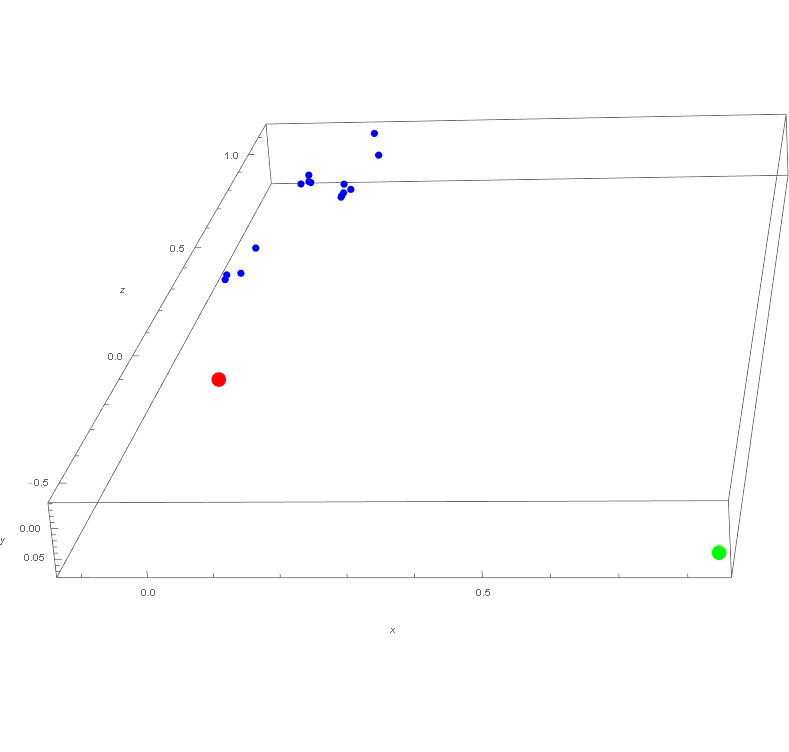
\includegraphics[width=\linewidth]{images/reconstructed_Points_Same_Resolutions.png}
	\caption{Rekonstruierte Szene, unskaliert in Pixeleinheiten}
	\label{fig:reconstructedSampson3D}
	\endminipage\hfill
	\minipage{0.48\textwidth}
	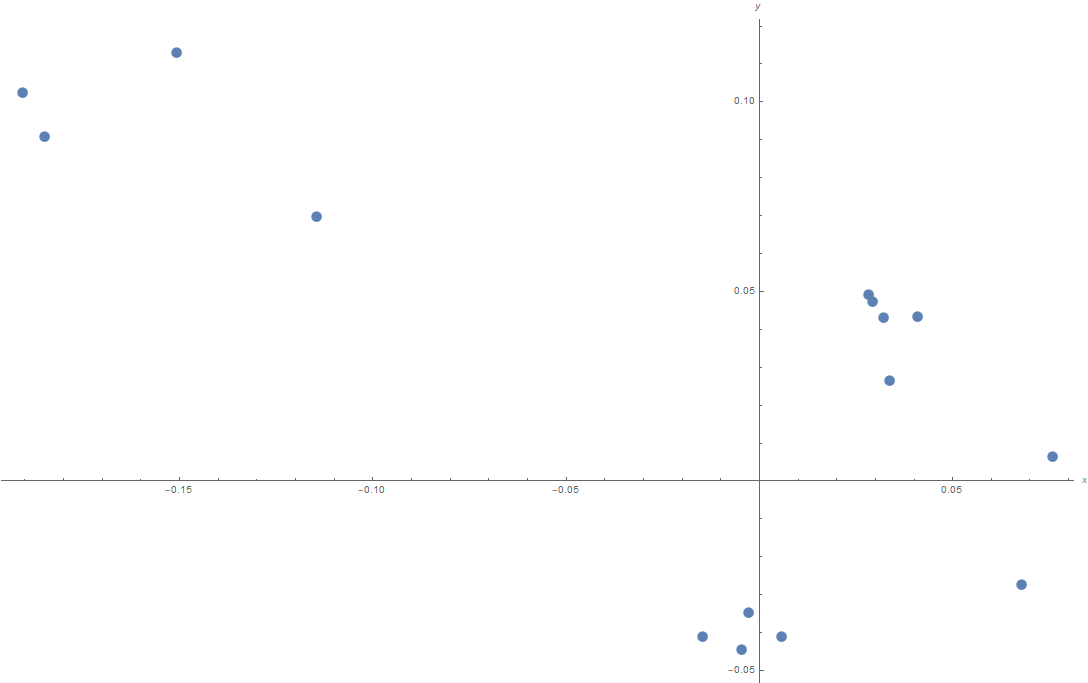
\includegraphics[width=\linewidth]{images/reconstructed_Points_Same_Resolutions2D.png}
	\caption{Rekonstruierte Szene, unskaliert, in Pixeleinheiten und in einem 2D-Plot angezeigt}
	\label{fig:reconstructedSampson2D}
	\endminipage\hfill
	%	\caption{Die mit dem \textit{SURF}-Algorithmus gefundenen Punkte sind mit den gelben Ziffern im Bild gekennzeichnet}
\end{figure}

%\begin{minipage}{\linewidth}
%	\centering
%	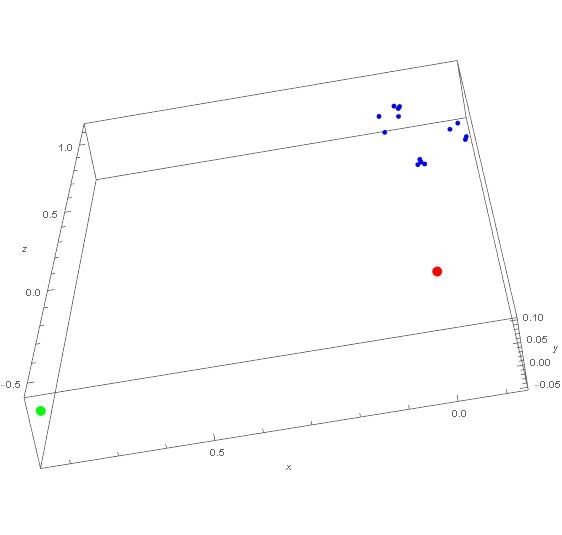
\includegraphics[width=.8\linewidth]{images/result_DetectedmathematicaPointsDifferentResolutions.png}
%	\captionof{figure}{Frafische Darstellung der optimalen Punkte $\hat{m}$ und $\hat{m'}$}
%\end{minipage}\\

%\subsection{andere Ansätze für Triangulationsverfahren}
%Um eine Triangulation zu ermöglichen, muss eine Methode gefunden werden, welche diesen Fehler so weit minimiert, dass es zu einer erfolgreichen Rückprojektion kommt. Die verwendete Methode zur Rekonstruktion der Szene wurde nach der Vorlage von \textit{Hartley \& Zisserman}\cite{HZ} implementiert und wird im folgenden Schritt für Schritt beschrieben.\\
%
%Voraussetzung ist, dass die Projektionsmatrizen $P$ und $P'$, sowie die Fundamentalmatrix $F$ bekannt sein müssen. Sind die Projektionsmatrizen $P$ und $P'$ bis auf eine projektive oder affine Komponenten bekannt, so ist es wünschenswert, wenn die Triangulierung auf einem affinen und projektiv invarianten Verfahren funktioniert\cite{HZ}.\\


%Die hier verwendeten Porjektionsmatrizen sind bis auf eine Skaleninvarianz genau bestimmt, was unter den Fall der affinen invarianz Fällt. Wären die intrinsischen Kameraparameter $K$ und $K'$ nicht bekannt gewesen, gibt es die Möglichkeit die Projektionsmatrizen über die Fundamentalmatrix $F$ mit dem, im Buch von \textit{Hartley \& Zisserman} beschriebenen  \textit{Stratified-Approach} bis auf eine projektive Invarianz genau zu bestimmen\cite{HZ}. 
%
%Die hier verwendete Triangulierung ist nur projektiv invariant, kann aber trotzdem genutzt werden. Die rekonstruierte Szene ist, dann wie im Minimalbeispiel auch, nicht auf ihre Originalmaße skaliert, was aber nach der Triangulierung noch getan werden kann.\\
%
%Die Triangulierung ist deshalb projektiv invariant, weil alle Rechenoperationen, wie die Minimierungen von Distanzen, sich nur auf die 2D-Bildern beziehen und sich nicht in den projektiven 3D-Raum erstreckt\cite{HZ}. \\
%
%Der Grundgedanke der Triangulation ist, dass zwei Punkte $\hat{m}$ und $\hat{m'}$ gefunden werden sollen, die möglichst nah an den ursprünglichen $m$ und $m'$ sind und gleichzeitig den \textit{Epipolar-Constraint} $\hat{x}'^TF\hat{x} = 0$ erfüllen. Dies erfolgt durch die Minimierung einer Kostenfunktion $C$.\\

% In vielen bekannten Computer Vision Applikationen wird für diese Minimierung eine numerische Lösung gewählt, die wohl bekannteste Methode ist der \textit{Levenberg-Marquardt} Algorithmus\cite{HZ}. Jedoch hat sich gezeigt, dass ein nahezu optimales Minimum der geometrischen Kostenfunktion $C$ auch durch eine Annäherung ersten Grades finden lässt. Die Annährung um die es sich handelt ist die sogenannten \textit{Sampson-approximation}


%\subsection{Minimieren der Kostenfunktion durch Sampson-approximation}

%
%Es sollen zwei Punkte $\hat{m}$ und $\hat{m}'$ gefunden werden, welche nahe an den Ursprünglichen $m$ und $m'$ liegen und gleichzeitig den \textit{Epipolar-Constraint} erfüllen. $\hat{m}$ und $\hat{m}'$ sollen durch Minimierung einer Kostenfunktion $C$ ermittelt werden, welche die Distanz  $d$ zwischen $m$ und $\hat{m}$ und $m'$ und $\hat{m'}$ minimiert.
%
%
%\begin{gather}
%	C(m,m') = d(m,\hat{m})^2 + d(m',\hat{m'})^2
%\end{gather}
%
%Die projizierten Punkte $\hat{m}$ und $\hat{m'}$ eines 3D-Objektpunktes $\hat{M}$ liegen auf einem paar korrespondierender Epipolarlinien. 



